\documentclass[journal,12pt,twocolumn]{IEEEtran}
\usepackage{cite}
\usepackage{amsmath,amssymb,amsfonts,amsthm}
\usepackage{algorithmic}
\usepackage{graphicx}
\usepackage{textcomp}
\usepackage{xcolor}
\usepackage{txfonts}
\usepackage{listings}
\usepackage{enumitem}
\usepackage{mathtools}
\usepackage{float}
\usepackage{gensymb}
\usepackage{comment}
\usepackage[breaklinks=true]{hyperref}
\usepackage{tkz-euclide} 
\usepackage{listings}
\usepackage{gvv}                                        
\def\inputGnumericTable{}                                 
\usepackage[latin1]{inputenc}                                
\usepackage{color}                                            
\usepackage{array}                                            
\usepackage{longtable}                                       
\usepackage{calc}            
\usepackage{multirow}                                         
\usepackage{hhline}                                           
\usepackage{ifthen}                                           
\usepackage{lscape}
\usepackage{amsmath}
\newtheorem{theorem}{Theorem}[section]
\newtheorem{problem}{Problem}
\newtheorem{proposition}{Proposition}[section]
\newtheorem{lemma}{Lemma}[section]
\newtheorem{corollary}[theorem]{Corollary}
\newtheorem{example}{Example}[section]
\newtheorem{definition}[problem]{Definition}
\newcommand{\BEQA}{\begin{eqnarray}}
\newcommand{\EEQA}{\end{eqnarray}}
\newcommand{\define}{\stackrel{\triangle}{=}}
\theoremstyle{remark}
\newtheorem{rem}{Remark}

\begin{document}

\bibliographystyle{IEEEtran}
\vspace{3cm}

\title{NCERT Discrete - 11.9.3.11}
\author{EE23BTECH11037 - M Esha$^{*}$}

\maketitle
\newpage
\bigskip

\renewcommand{\thefigure}{\theenumi}
\renewcommand{\thetable}{\theenumi}

\vspace{3cm}
\textbf{Question 11.9.3.11:}

Evaluate $\sum_{k=1}^{11} (2 + 3^k)$.

\solution
\begin{table}[h!]
  \centering
  \begin{tabular}{|c|c|c|}
   \hline
   variable&value&description  \\
   \hline
   $x(0)$ & $3$ & first term of the geometric progession\\
   \hline
   $r$ & $3$ & common ratio of the geometeric progression\\
   \hline
   $x(n)$ & $3^{n}u\brak{n}$& $n^{th}$ term of the geometric progession\\
   \hline
   $y(n)$ &$\frac{x(0)(r^{n+1}-1)}{r-1}u\brak{n}$ &Sum of the n term of the geometric progression\\
   \hline 
\end{tabular}


  \caption{Input Parameters}
    \label{tab:table1}
\end{table}

\begin{align}
x\brak{n} &= {2+3^{n}}u(n)\\
X\brak{z} &= \frac{2}{{1-z^{-1}}}+\frac{1}{1-3z^{-1}} , \quad|z| > 1\\
y\brak{n} &= x\brak{n}*u\brak{n} \\
Y\brak{z} &= X\brak{z}U\brak{z}\\
&=\frac{2}{\brak{1-z^{-1}}^{2}}+\brak{\frac{1}{\brak{1-3z^{-1}}\brak{1-z^{-1}}}} ,\quad|z| >{1}\\
&=\frac{2}{\brak{1-z^{-1}}^{2}}+\brak{\frac{1}{2}}\brak{\brak{\frac{3}{1-3z^{-1}}}-\brak{\frac{1}{1-z^{-1}}}}
\end{align}
 Using Contour Integration to find the inverse $Z$-transform,
\begin{align}
y(10)&=\frac{1}{2\pi j}\oint_{C}Y(z) \;z^{9} \;dz  \\
&=\frac{1}{2\pi j}\oint_{C}\brak{\frac{2}{\brak{1-z^{-1}}^{2}}+\brak{\frac{1}{2}}\brak{\frac{3}{1-3z^{-1}}-\frac{1}{1-z^{-1}}}}{z^{9}}\,dz\\
R &=\frac{1}{\brak {m-1}!}\lim\limits_{z\to a}\frac{d^{m-1}}{dz^{m-1}}\brak {{(z-a)^{m}}f\brak{z}}
\end{align}
For $R_1$ , $m=2$ :
\begin{align}
R_1 &=\frac{1}{\brak {1}!}\lim\limits_{z\to 1}\frac{d}{dz}\brak {{\brak{z-1}^{2}}\frac{2z^{10}}{{\brak{z-1}^2}}}  \\
&=2\lim\limits_{z\to 1}\frac{d}{dz}(z^{10})   \\
&=20
\end{align}
For $R_2$ , $m=1$:
\begin{align}
R_2 &=\frac{1}{\brak {0}!}\lim\limits_{z\to 3}\frac{1}{2}\brak {{z-3}\frac{3z^{11}}{{{z-3}}}} \\
&=\frac{1}{2}{3^{12}}  \\
&=265720.5
\end{align}
For $R_3$ , $m=1$ :
\begin{align}
R_3 &=\frac{1}{\brak {0}!}\lim\limits_{z\to 1}\brak{\frac{1}{2}\brak {{z-1}\frac{z^{11}}{{{z-1}}}}}  \\
&=\frac{1}{2}\lim\limits_{z\to1}z^{11}
&=0.5\\
 R_1 + R_2 + R_3 &= 265741\\
    \implies  y{(10)} &= 265741
\end{align}
\begin{figure}[b]
    \centering
    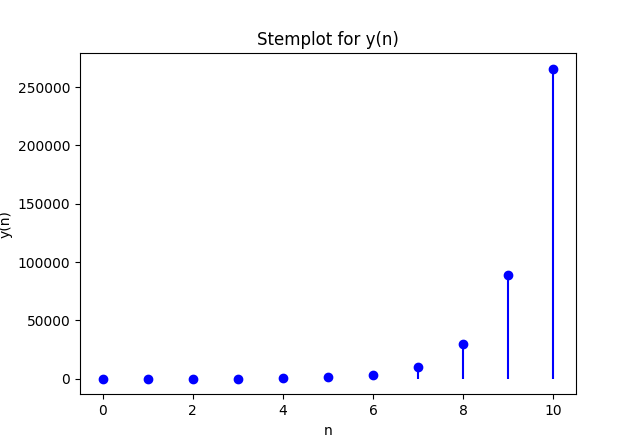
\includegraphics[width=\columnwidth]{11/9/3/11/figs/1.png}
    \caption{stem plot }
    \label{fig:1}
\end{figure}
\end{document}
